% arara: latex: { interaction: nonstopmode, options: ['-halt-on-error'] }
% arara: dvisvgm: { options: ['--no-fonts', '--exact-bbox', '--zoom=-1'] }
% Expands the i=4 rebuild in smallest-enclosing-circle2.tex.
% Exact intermediate radius squared: 13/4; final radius squared: 169/36.
\documentclass[tikz,border=8pt,11pt]{standalone}
\usepackage{amsmath,amssymb}
\definecolor{circleblue}{HTML}{0072B2}
\definecolor{pointred}{HTML}{D55E00}
\definecolor{fixedpurple}{HTML}{8B4C9D}
\definecolor{ink}{HTML}{25313C}
\definecolor{muted}{HTML}{7C8792}
\tikzset{
  current/.style={draw=circleblue,line width=1.1pt,fill=circleblue!6},
  previous/.style={draw=muted,dashed,line width=0.9pt},
  point label/.style={font=\small,inner sep=4pt,text=ink},
}

% All four points are shown as context, even before the inner scan reaches them.
% The argument selects the point currently being tested (0 means none).
\newcommand{\points}[1]{%
  \foreach \id/\px/\py/\anchor in {
    1/-2/0/north east,2/2/0/north west,3/0/1/west,4/0/3/south}{%
    \ifnum\id=#1\relax
      \fill[pointred] (\px,\py) circle[radius=3pt];
      \node[point label,text=pointred,anchor=\anchor] at (\px,\py) {$P_{\id}$};
    \else
      \fill[ink] (\px,\py) circle[radius=2.3pt];
      \node[point label,anchor=\anchor] at (\px,\py) {$P_{\id}$};
    \fi
  }%
}
\newcommand{\fixed}[2]{%
  \draw[fixedpurple,line width=1.2pt] (#1,#2) circle[radius=5.2pt];
}

\begin{document}
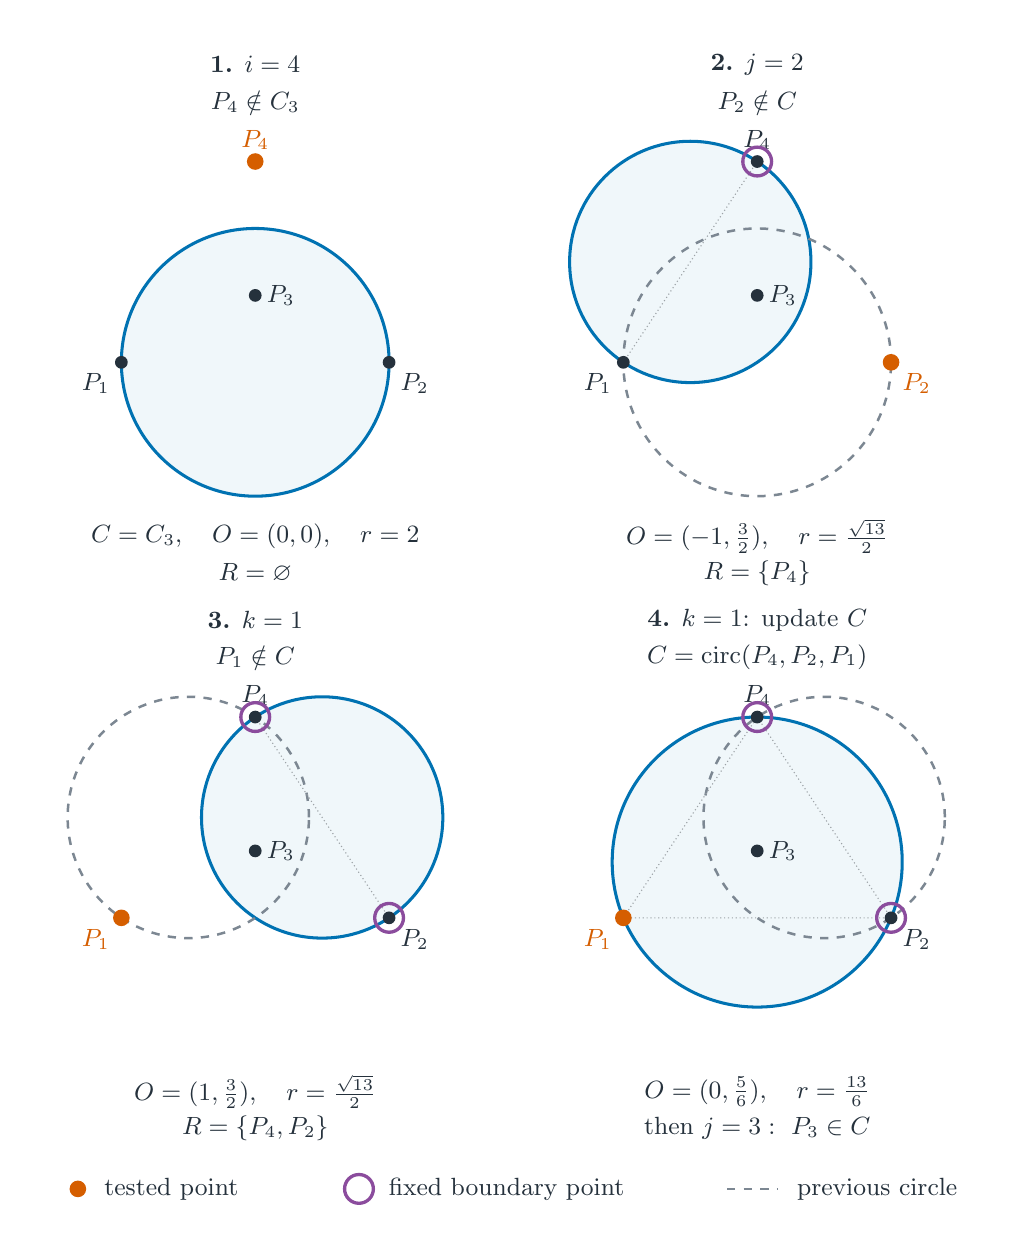
\begin{tikzpicture}[x=0.85cm,y=0.85cm,font=\small,text=ink]
  \fill[white] (-3.4,-12.85) rectangle (10.9,5);

  \begin{scope}
    \node at (0,4.45) {\textbf{1.} $i=4$};
    \node at (0,3.9) {$P_4\notin C_3$};
    \draw[current] (0,0) circle[radius=2];
    \points{4}
    \node at (0,-2.6) {$C=C_3,\quad O=(0,0),\quad r=2$};
    \node at (0,-3.15) {$R=\varnothing$};
  \end{scope}

  \begin{scope}[xshift=6.375cm]
    \node at (0,4.45) {\textbf{2.} $j=2$};
    \node at (0,3.9) {$P_2\notin C$};
    \draw[current] (-1,{3/2}) circle[radius={sqrt(13)/2}];
    \draw[previous] (0,0) circle[radius=2];
    \draw[ink!45,densely dotted] (-2,0) -- (0,3);
    \points{2}
    \fixed{0}{3}
    \node at (0,-2.6) {$O=(-1,\tfrac32),\quad r=\tfrac{\sqrt{13}}2$};
    \node at (0,-3.15) {$R=\{P_4\}$};
  \end{scope}

  \begin{scope}[yshift=-7.055cm]
    \node at (0,4.45) {\textbf{3.} $k=1$};
    \node at (0,3.9) {$P_1\notin C$};
    \draw[current] (1,{3/2}) circle[radius={sqrt(13)/2}];
    \draw[previous] (-1,{3/2}) circle[radius={sqrt(13)/2}];
    \draw[ink!45,densely dotted] (2,0) -- (0,3);
    \points{1}
    \fixed{0}{3}
    \fixed{2}{0}
    \node at (0,-2.6) {$O=(1,\tfrac32),\quad r=\tfrac{\sqrt{13}}2$};
    \node at (0,-3.15) {$R=\{P_4,P_2\}$};
  \end{scope}

  \begin{scope}[xshift=6.375cm,yshift=-7.055cm]
    \node at (0,4.45) {\textbf{4.} $k=1$: update $C$};
    \node at (0,3.9) {$C=\operatorname{circ}(P_4,P_2,P_1)$};
    \draw[current] (0,{5/6}) circle[radius={13/6}];
    \draw[previous] (1,{3/2}) circle[radius={sqrt(13)/2}];
    \draw[ink!45,densely dotted] (-2,0) -- (2,0) -- (0,3) -- cycle;
    \points{1}
    \fixed{0}{3}
    \fixed{2}{0}
    \node at (0,-2.6) {$O=(0,\tfrac56),\quad r=\tfrac{13}{6}$};
    \node at (0,-3.15) {then $j=3:\ P_3\in C$};
  \end{scope}

  \fill[pointred] (-2.65,-12.35) circle[radius=3pt];
  \node[anchor=west] at (-2.4,-12.35) {tested point};
  \draw[fixedpurple,line width=1.2pt] (1.55,-12.35) circle[radius=5.2pt];
  \node[anchor=west] at (1.85,-12.35) {fixed boundary point};
  \draw[previous] (7.05,-12.35) -- (7.8,-12.35);
  \node[anchor=west] at (7.95,-12.35) {previous circle};
\end{tikzpicture}
\end{document}
